\subsection{Main Challenges}\label{subsec:introduction--main-challenges}

The three fundamental properties we just discussed (concurrency, no global clock, partial failures) tell us \textbf{why distributed systems are intrinsically difficult}. Now we move to the practical engineering question: \emph{what problems must we solve when actually building one?} We can identify seven main challenges: heterogeneity, openness, security, scalability, failure handling, concurrency, and transparency.

\highspace
In this section, we will discuss the first six challenges, because they try to \textbf{cope the difficulties created by distribution}. Instead, transparency, even though it is a challenge, is more of a \textbf{design objective} because it decides how much of the underlying distribution is exposed to the user or programmer. We will discuss transparency in next section.

\begin{figure}[!htp]
    \centering
    \tikzsetnextfilename{introduction--main-challenges}
    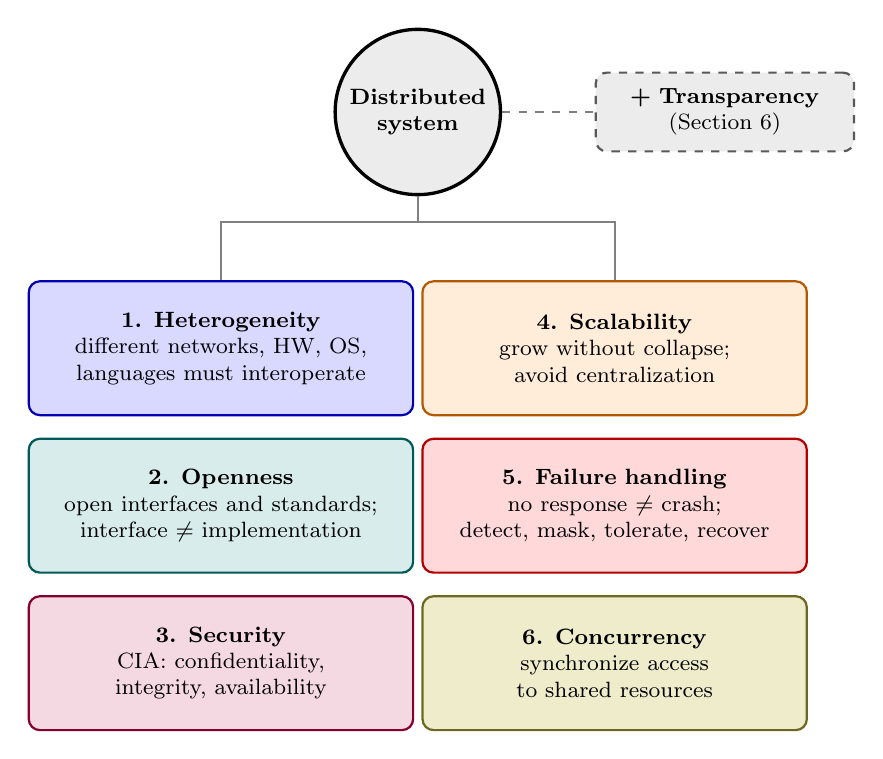
\begin{tikzpicture}[
            font=\footnotesize,
            challenge/.style={
                rounded corners=4pt, draw=#1!70!black, fill=#1!15, thick,
                text width=4.6cm, minimum height=1.7cm,
                align=center, inner sep=4pt
            },
            core/.style={
                circle, draw=black, fill=gray!15, very thick,
                align=center, font=\bfseries\footnotesize, inner sep=3pt
            },
            link/.style={gray, thick}
        ]

        % --- Top ---
        \node[core] (ds) at (0,0) {Distributed\\system};
        \node[challenge=gray, dashed, text width=3cm, minimum height=1cm] (tra) at (3.9,0)
        {\textbf{+ Transparency}\\(Section 6)};
        \draw[link, dashed] (ds) -- (tra);

        % --- Six challenges, two columns ---
        \node[challenge=blue]   (het) at (-2.5,-3.0)
        {\textbf{1. Heterogeneity}\\different networks, HW, OS,\\languages must interoperate};
        \node[challenge=teal]   (op)  at (-2.5,-5.0)
        {\textbf{2. Openness}\\open interfaces and standards;\\interface $\neq$ implementation};
        \node[challenge=purple] (sec) at (-2.5,-7.0)
        {\textbf{3. Security}\\CIA: confidentiality,\\integrity, availability};

        \node[challenge=orange] (sca) at (2.5,-3.0)
        {\textbf{4. Scalability}\\grow without collapse;\\avoid centralization};
        \node[challenge=red]    (fai) at (2.5,-5.0)
        {\textbf{5. Failure handling}\\no response $\neq$ crash;\\detect, mask, tolerate, recover};
        \node[challenge=olive]  (con) at (2.5,-7.0)
        {\textbf{6. Concurrency}\\synchronize access\\to shared resources};

        % --- Connectors ---
        \draw[link] (ds.south) -- (0,-1.4) -| (het.north);
        \draw[link] (ds.south) -- (0,-1.4) -| (sca.north);

    \end{tikzpicture}
    \caption{Main challenges of distributed systems.}
\end{figure}

\newpage

\begin{flushleft}
    \textcolor{Red2}{\faIcon{shapes} \textbf{Heterogeneity}}
\end{flushleft}
\textbf{Heterogeneity} means that the \hl{components} of a distributed system may be fundamentally \hl{different from one another}. A distributed system may connect different networks, hardware, operating systems, programming languages, and so on. Yet all of them are expected to communicate correctly. That is the \textbf{challenge}.
\begin{itemize}
    \item \important{Network heterogeneity}. Even if everything uses TCP/IP, the \hl{underlying networks can be very different.} For example, wired Ethernet, wireless Wi-Fi, wireless ad-hoc networks. TCP/IP can hide many differences at higher levels, but it cannot make the underlying physical environments identical.

    \item \important{Hardware heterogeneity}. Now suppose two machines have different architectures. For example, one is x86 and the other is ARM. Imagine one machine sends a binary representation of a value to another. \hl{If both machines interpret that sequence of bytes differently, communication breaks}. Therefore, distributed communication needs \textbf{agreed representations}.

    \item \important{Operating-system heterogeneity}. Different machines may run different operating systems (e.g., Linux, Windows, macOS). The networking functionality may ultimately be similar, but the APIs and semantics exposed to applications can differ. So if a distributed application relies too heavily on one platform's behavior, \textbf{portability becomes difficult}.

    \item \important{Programming-language heterogeneity}. Suppose a three component distributed system has one component written in C, another in Java, and the third in Python. Each language has its own data types, memory management, and runtime behavior. \hl{If these components need to exchange complex data structures, we must define a common serialization format and ensure that each language can correctly encode and decode it.}
\end{itemize}
So the core challenge is: \emph{\textbf{how do heterogeneous components interoperate?}} This is precisely one of the problems middleware can help with.

\newpage

\begin{flushleft}
    \textcolor{Red2}{\faIcon{door-open} \textbf{Openness}}
\end{flushleft}
\textbf{Openness} is about whether the distributed system can be extended, reimplemented, and integrated with other systems. The central idea is that \hl{other components must know how to interact with the system.} That \textbf{requires clearly defined rules}.
\begin{itemize}
    \item \important{Publish protocols and interfaces}. Suppose we build a service $S$. If nobody knows which messages it accepts, what those messages mean, what responses it return, then nobody else can implement a compatible client.

        \highspace
        So an open system needs published \textbf{protocols} and \textbf{service interfaces}. Note that \hl{same interface does \textbf{not} imply same implementation.} For example, two different implementations of a web server can both support the same HTTP protocol and serve the same content, but they may have different internal architectures and optimizations.

    \item \important{Interoperability}. Suppose company $A$ implements a client and company $B$ implements a server. If both follow the same standard, they should be able to work together. That property is called \textbf{interoperability}. \hl{Different implementations of the same protocol should be able to communicate correctly}, even if they are built by different teams, in different languages, and on different platforms.

    \item \important{Portability}. Openness should also help software move between environments. For example, if an application depends on a standardized abstraction rather than proprietary low-level details, it becomes easier to move it from one platform to another. So:
        \begin{itemize}
            \item \textbf{Interoperability} concerns different systems working together;
            \item \textbf{Portability} concerns moving software between environments.
        \end{itemize}

    \item \important{Standards}. To achieve openness, standards are extremely useful. Instead of every organization inventing its own protocols, we agree on \textbf{common standard}. Then independent implementations can cooperate.

        The internet is the classic example. Internet protocols are specified through \textbf{RFCs}, and the \textbf{IETF} provides an open standardization process. This is one major reason completely different devices can communicate over the internet.
\end{itemize}
We can summarize the openness idea as: \hl{specify what components must do, not how they must be implemented.}

\newpage

\begin{flushleft}
    \textcolor{Red2}{\faIcon{lock} \textbf{Security}}
\end{flushleft}
Distribution greatly increases the \textbf{security problem} because resources are accessed through a network.
In a centralized machine, many resources may be protected by the physical and operating-system boundary.
In a distributed system:
\begin{equation*}
    \text{Client}
    \xrightarrow{\text{network}}
    \text{Server}
\end{equation*}
And potentially anyone connected to that network may attempt to interact with the service.

\highspace
The three main security properties that we want to achieve are called the \textbf{CIA triad}:
\begin{equation*}
    C = \text{Confidentiality},\qquad
    I = \text{Integrity},\qquad
    A = \text{Availability}
\end{equation*}

\begin{figure}[!htp]
    \centering
    \tikzsetnextfilename{security--cia-triad}
    \begin{tikzpicture}[
            font=\footnotesize,
            execute at begin node={\hyphenpenalty=10000 \exhyphenpenalty=10000 },
            card/.style={
                rounded corners=5pt, draw=purple!70!black, fill=purple!10, thick,
                text width=3.6cm, minimum height=1.65cm, align=center, inner sep=4pt
            },
            core/.style={
                circle, draw=purple!80!black, fill=purple!20, very thick,
                align=center, font=\footnotesize, inner sep=5pt
            },
            arr/.style={
                <->, very thick, purple!75!black, >=Stealth
            },
            link/.style={
                thick, purple!35, dashed
            }
        ]

        % Coordinates for the 3 vertices
        \coordinate (tc) at (0, 2.4);
        \coordinate (lc) at (-3.4, -1.4);
        \coordinate (rc) at (3.4, -1.4);

        % Central Core Badge
        \node[core] (core) at (0, -0.15) {
            \textcolor{purple!80!black}{\faIcon{shield-alt}}\\[2pt]
            \textbf{CIA Triad}\\[-2pt]
            {\scriptsize\color{gray!70!black} Security}
        };

        % Vertex 1: Confidentiality (Top)
        \node[card] (c) at (tc) {
            \textbf{\textcolor{purple!80!black}{\faIcon{lock}} Confidentiality (C)}\\[2pt]
            {\scriptsize\bfseries\color{purple!90!black}``Can an attacker read?''}\\[2pt]
            {\scriptsize\color{gray!80!black}protect against disclosure\\$\rightarrow$ \textit{encryption}}
        };

        % Vertex 2: Integrity (Bottom-Left)
        \node[card] (i) at (lc) {
            \textbf{\textcolor{purple!80!black}{\faIcon{fingerprint}} Integrity (I)}\\[2pt]
            {\scriptsize\bfseries\color{purple!90!black}``Can an attacker alter?''}\\[2pt]
            {\scriptsize\color{gray!80!black}protect against tampering\\$\rightarrow$ \textit{checksums, signatures}}
        };

        % Vertex 3: Availability (Bottom-Right)
        \node[card] (a) at (rc) {
            \textbf{\textcolor{purple!80!black}{\faIcon{server}} Availability (A)}\\[2pt]
            {\scriptsize\bfseries\color{purple!90!black}``Is the system usable?''}\\[2pt]
            {\scriptsize\color{gray!80!black}protect against DoS\\$\rightarrow$ \textit{redundancy, replication}}
        };

        % Central radial dashed links
        \draw[link] (core) -- (c);
        \draw[link] (core) -- (i);
        \draw[link] (core) -- (a);

        % Triangle perimeter arrows connecting the nodes directly
        \draw[arr] (c) -- (i);
        \draw[arr] (c) -- (a);
        \draw[arr] (i) -- (a);

    \end{tikzpicture}
    \caption{The CIA triad: core security objectives in distributed systems.}
\end{figure}

\noindent
Where:
\begin{itemize}
    \item \important{Confidentiality} means that \hl{information is accessible only to authorize entities.}

        \begin{examplebox}[: Confidentiality]
            Suppose Alice sends a \emph{password} to a remote server. Without protection, an attacker could intercept the message and read the password. We therefore want that an unauthorized observer cannot learn the content of the message.

            So confidentiality protects against \textbf{unauthorized disclosure}. Encryption is one major mechanism used to achieve this.
        \end{examplebox}

    \item \important{Integrity} means \hl{protecting information against \textbf{unauthorized alteration or corruption}.}

        \begin{examplebox}[: Integrity]
            Suppose Alice sends a message ``\texttt{transfer 10\euro}'' to Bob. An attacker should not be able to transform it into ``\texttt{transfer 1000\euro}'' without being detected.

            So confidentiality ask ``\emph{can an attacker read the information?}'', but integrity asks ``\emph{can an attacker change the information?}''.
        \end{examplebox}

    \item \important{Availability} means that \hl{legitimate users must be able to access the resource.}

        \begin{examplebox}[: Availability]
            An attacker may not steal or modify anything and still successfully attack the system by preventing others from using it. For example, this is the idea behind \textbf{Denial of Service (DoS)} attacks, where the attacker floods a server with requests so that legitimate users cannot get through.

            Suppose the server can process 1000 requests per second and an attacker generates 1 million requests per second. Legitimate requests may become impossible to serve.

            So \textbf{security is not only about secrecy}, but also about \textbf{ensuring that the system remains usable}.
        \end{examplebox}
\end{itemize}

\newpage

\begin{flushleft}
    \textcolor{Red2}{\faIcon{expand-arrows-alt} \textbf{Scalability}}
\end{flushleft}
A distributed system is \textbf{scalable} if we can \hl{increase its size without causing an unacceptable degradation in performance.} But ``size'' has more than one meaning. There are \textbf{three dimensions of scalability}:
\begin{itemize}
    \item \important{Scaling users and resources}. The simplest case is increasing the number of users, machines, services, or data. A scalable architecture should not collapse simply because the number of participants grows. The fundamental challenge is therefore \hl{reconcile increasing scale with acceptable performance.} It is easy to build something that works for 10 machines. The difficulty is designing it so that adding another 10,000 machines does not fundamentally break the architecture.

    \item \important{Geographic scalability}. A system may also grow geographically (e.g., from a single data center to multiple data centers across the world) and the physical distance becomes relevant. So geographic growth introduces new challenges, such as \textbf{latency} and \textbf{fault tolerance}. For example, if a system is designed to operate within a single data center, it may not handle the increased latency and potential failures that come with a global distribution.

    \item \important{Administrative scalability}. A small distributed system may be completely controlled by \textbf{one organization}. But as the system grows, it may involve multiple organizations, each with its own policies, procedures, and administrative domains. So scalability is not merely ``\emph{can we add more servers?}'', but also \hl{``\emph{can the system grow in users, geography, and administrative domains?}''}
\end{itemize}
\textcolor{Red2}{\faIcon{exclamation-triangle} \textbf{The enemy of scalability: Centralization.}} In general, \hl{centralized components tend to become scalability bottlenecks.} There are three typical forms of centralization:
\begin{enumerate}
    \item \important{Centralized services}. Suppose every user must contact one server:
        \begin{equation*}
            \begin{array}{ccccc}
                C_1&C_2&C_3&\cdots&C_n\\
                &\searrow&\downarrow&\swarrow\\
                &&\boxed{S}
            \end{array}
        \end{equation*}
        As $n$ grows, server $S$ eventually becomes overloaded, a performance bottleneck, potentially a single point of failure. So \hl{one server for everybody does not scale indefinitely.}

    \item \important{Centralized data}. Suppose the entire distributed system depends on one global directory: one online telephone book, one DNS server, one global database. Then, every operation requires querying it. Again:
        \begin{equation*}
            \text{more machines}
            \Rightarrow
            \text{more requests to the same data source}
        \end{equation*}
        Eventually the \hl{centralized data structure becomes the bottleneck.}

    \item \important{Centralized algorithms}. Imagine an algorithm that makes decisions using the \textbf{complete state of the entire system}. For example, a routing algorithm that:
        \begin{equation*}
            \text{collect information about every node}
            \rightarrow
            \text{compute routing decision}
        \end{equation*}
        With 5 machines, obtaining complete information may be easy, but with $10^6$ machines, maintaining an always-up-to-date global view can become extremely expensive or unrealistic.

        So \hl{scalability requires us to be suspicious} not only of centralized servers, but also of \hl{algorithms that conceptually require complete global knowledge.}
\end{enumerate}
\textcolor{Green3}{\faIcon{check-circle} \textbf{Decentralized algorithms.}} Due to the scalability problems of centralized algorithms, we often prefer \textbf{decentralized algorithms}. There are four properties worth remembering:
\begin{enumerate}
    \item \hl{No machine has complete information.} Instead of one machine knowing everything, each machine only knows a part of the system's state.

    \item \hl{Decisions use local information.} A node makes decisions based on the information available to it, rather than first collecting the complete global state. This reduces coordination overhead.

    \item \hl{One machine failing should not destroy the algorithm.} The algorithm should be robust to failures, so that the failure of a single node does not prevent the system from functioning.

    \item \hl{No implicit global-clock assumption.} The algorithm should not rely on the existence of a global clock or synchronized time across machines, as this is often unrealistic in distributed systems (as discussed in previous sections).
\end{enumerate}
\textcolor{Green3}{\faIcon{tools} \textbf{Techniques for scalability.}} Several techniques can help achieve scalability:
\begin{itemize}
    \item \textcolor{Green3}{\textbf{Asynchronous communication}}. Instead of waiting for a response, a node can continue processing other tasks. This allows the system to handle more requests concurrently.

    \item \textcolor{Green3}{\textbf{Caching and replication}}. Instead of forcing everybody to retrieve data from one place, we can replicate data across multiple nodes and cache frequently accessed data. Of course, replication introduces a new problem: \emph{\textbf{how do we keep the copies consistent?}} That will become an entire topic of its own in later sections.

    \item \textcolor{Green3}{\textbf{Epidemic dissemination}}. The name is intentionally evocative: information spreads like a virus. Instead of one node sending information to all others, it sends it to a few neighbors, which then send it to their neighbors, and so on. This can be more efficient than flooding the network with messages.

    \item \textcolor{Green3}{\textbf{Hierarchical structuring}}. Instead of organizing millions of components in one flat structure, we divide them hierarchically. Then many operations can be performed locally within a sub-hierarchy, reducing the need for global coordination.
\end{itemize}
However, in general the \textbf{principle} is: \hl{global knowledge and global coordination become increasingly expensive as a system grows.} Therefore scalable distributed systems tend toward \textbf{decentralization, local decisions, and distribution of data/workload.}

\begin{figure}[htbp]
    \centering
    \tikzsetnextfilename{scalability}
    \begin{tikzpicture}[
            font=\footnotesize,
            execute at begin node={\hyphenpenalty=10000 \exhyphenpenalty=10000 },
            root/.style={
                rounded corners=4pt, draw=orange!70!black, fill=orange!25, very thick,
                text width=10.0cm, align=center, inner sep=5pt
            },
            dim/.style={
                rounded corners=4pt, draw=orange!70!black, fill=orange!12, thick,
                text width=3.2cm, minimum height=1.3cm, align=center, inner sep=3pt
            },
            bad/.style={
                rounded corners=4pt, draw=red!70!black, fill=red!10, thick,
                text width=3.2cm, minimum height=1.3cm, align=center, inner sep=3pt
            },
            bottleneck/.style={
                rounded corners=4pt, draw=red!70!black, fill=red!25, very thick,
                text width=10.0cm, align=center, inner sep=4pt
            },
            tech/.style={
                rounded corners=4pt, draw=green!50!black, fill=green!12, thick,
                text width=2.3cm, minimum height=1.5cm, align=center, inner sep=3pt
            },
            band/.style={
                rounded corners=8pt, draw=#1!50, fill=#1!5, thick, inner sep=6pt
            },
            sect/.style={font=\scriptsize\bfseries, text=#1!70!black, anchor=west},
            arr/.style={-{Stealth[length=2.5mm]}, thick, gray!70!black},
            flow/.style={font=\scriptsize\itshape, text=gray!60!black, anchor=west}
        ]

        % ================= ROOT =================
        \node[root] (root) at (0,0)
        {\textbf{Scalability:} grow without unacceptable performance loss};

        % ================= BAND 1: dimensions =================
        \node[sect=orange] (l1) at (-5.2,-1.1) {GROW IN THREE DIMENSIONS};
        \node[dim] (d1) at (-3.6,-2.25) {\textbf{Users/resources}\\more users,\\machines, data};
        \node[dim] (d2) at (0,-2.25)    {\textbf{Geography}\\from one site\\to worldwide};
        \node[dim] (d3) at (3.6,-2.25)  {\textbf{Administration}\\more organizations\\and policies};

        % ================= BAND 2: centralization =================
        \node[sect=red] (l2) at (-5.2,-4.08) {ENEMY: CENTRALIZATION};
        \node[bad] (c1) at (-3.6,-5.2) {\textbf{Services}\\one server\\for everybody};
        \node[bad] (c2) at (0,-5.2)    {\textbf{Data}\\one global\\directory};
        \node[bad] (c3) at (3.6,-5.2)  {\textbf{Algorithms}\\need complete\\global state};
        \node[bottleneck] (bn) at (0,-6.7) {\textbf{Bottleneck} (and single point of failure)};
        \foreach \n in {c1,c2,c3}
        \draw[arr, red!70!black] (\n.south) -- (\n.south |- bn.north);

        % ================= BAND 3: techniques =================
        \node[sect=green] (l3) at (-5.2,-8.28) {REMEDY: DECENTRALIZE, USE LOCAL INFORMATION};
        \node[tech] (t1) at (-3.9,-9.55) {\textbf{Asynchronous}\\don't wait\\for replies};
        \node[tech] (t2) at (-1.3,-9.55) {\textbf{Caching and}\\\textbf{replication}\\copies near users};
        \node[tech] (t3) at (1.3,-9.55)  {\textbf{Epidemic}\\nodes spread\\info to nodes};
        \node[tech] (t4) at (3.9,-9.55)  {\textbf{Hierarchy}\\keep operations\\local};

        % ================= BANDS (background) =================
        \begin{scope}[on background layer]
            \node[band=orange, fit=(l1)(d1)(d2)(d3)] (cl1) {};
            \node[band=red,    fit=(l2)(c1)(c2)(c3)(bn)] (cl2) {};
            \node[band=green,  fit=(l3)(t1)(t2)(t3)(t4)] (cl3) {};
        \end{scope}

        % ================= CENTRAL FLOW =================
        \draw[arr, very thick] (root.south) -- (cl1.north);
        \draw[arr, very thick] (cl1.south) -- (cl2.north)
        node[flow, pos=0.5, xshift=2pt] {but centralized designs do not grow};
        \draw[arr, very thick] (cl2.south) -- (cl3.north)
        node[flow, pos=0.5, xshift=2pt] {so we avoid centralization};

    \end{tikzpicture}
    \caption{Scalability: dimensions, enemy and remedies.}
\end{figure}

\newpage

\begin{flushleft}
    \textcolor{Red2}{\faIcon{life-ring} \textbf{Failure Handling}}
\end{flushleft}
We already encountered \textbf{partial failures} as a fundamental property. Now the question becomes: ``\emph{what can the system actually do about failures?}''. And partial failures are \hl{problematic} precisely because \hl{some components may continue operating while others fail:}
\begin{equation*}
    A:\checkmark
    \qquad
    B:\times
    \qquad
    C:\checkmark
\end{equation*}
The system has to decide how to behave in this intermediate state. Usually, the system applies the following four strategies:
\begin{equation*}
    \text{detection}
    \rightarrow
    \text{masking}
    \rightarrow
    \text{tolerance}
    \rightarrow
    \text{recovery}
\end{equation*}
Plus \textbf{redundancy}. These are related, but they are \textbf{not synonyms}.
\begin{enumerate}
    \item \important{Detecting failures}. Some failures are \textbf{easy to detect}.

        \begin{examplebox}[: Easy failure detection]
            Suppose a received message is corrupted. A checksum can reveal:
            \begin{equation*}
                \text{received data} \neq \text{expected valid data}
            \end{equation*}
            So we know a failure occurred.
        \end{examplebox}

        But other failures are fundamentally \textbf{harder}.

        \begin{examplebox}[: Hard failure detection]
            Suppose a client sends a request to a server, but the server does not respond. Is the server down? Or is the network just slow? Or did the response get lost? \hl{We cannot distinguish between these cases with certainty.} This is a central distributed-systems issue.
        \end{examplebox}

        For some remote failures, we cannot detect them \textbf{with certainty}, we can only \textbf{suspect} that they occurred. So the challenge becomes \hl{manage failures that cannot always be definitively detected.}

    \item \important{Masking failures}. Sometimes, once a failure is detected, we can prevent the application from noticing it. This is called \textbf{failure masking}.

        \begin{examplebox}[: Failure masking]
            Suppose a message fails to arrive. We can retransmit and if the second transmission succeeds, the user may never notice that the first message was lost.
        \end{examplebox}

        So \hl{masking means hiding the effect of a failure.} The failure happened, but we simply prevented it from becoming visible at the higher level.

    \item \important{Tolerating failures}. Not every failure can be completely hidden. Sometimes the system instead continues operating despite the failure. This is called \textbf{fault tolerance}.

        \begin{examplebox}[: Fault tolerance]
            Suppose a distributed service normally provides:
            \begin{equation*}
                \{A,B,C,D\}
            \end{equation*}
            But one component fails.
            Perhaps the system can continue providing:
            \begin{equation*}
                \{A,B,C\}
            \end{equation*}
            While temporarily losing functionality $D$.
        \end{examplebox}

        Fault tolerance is based on \textbf{degraded service}, because \hl{reduced functionality is preferable to complete failure.} The system may not be able to provide everything, but it can still provide something.

    \item \important{Recovering from failures}. Eventually we may want the failed component to return to a valid state. One basic technique is periodically storing its state on permanent storage. Suppose the component evolves:
        \begin{equation*}
            S_0\rightarrow S_1\rightarrow S_2\rightarrow S_3
        \end{equation*}
        And periodically persists:
        \begin{equation*}
            S_2
            \rightarrow
            \boxed{\text{stable storage}}
        \end{equation*}
        Then the component crashes while in $S_3$:
        \begin{equation*}
            S_3\times
        \end{equation*}
        After restarting, we may restore:
        \begin{equation*}
            \boxed{S_2}
        \end{equation*}
        Rather than starting from nothing. So \hl{recovery restores a component to a usable state after failure.} The fact that the overall application state is distributed makes recovery considerably more \textbf{complicated} than simply restarting one process, but that deeper problem comes later.
\end{enumerate}
\textcolor{Green3}{\faIcon{check-circle} \textbf{Redundancy.}} One of the most common ways to mask or tolerate failures is redundancy. Instead of having:
\begin{equation*}
    \boxed{\text{Server}_A}
\end{equation*}
We may have:
\begin{equation*}
    \boxed{\text{Server}_A}
    \qquad
    \boxed{\text{Server}_B}
    \qquad
    \boxed{\text{Server}_C}
\end{equation*}
If:
\begin{equation*}
    \text{Server}_A\times
\end{equation*}
Another server may continue providing the service. This is \textbf{replicated servers}. And the same concept applies to communication paths providing \textbf{redundant routes}, or to data storage providing \textbf{replicated data}. So redundancy means: \hl{do not make the system depend on a single instance of a critical resource.} But there is an important warning, because \textbf{keeping replicas in a distributed system is not easy}. If we have multiple copies of a resource, we must ensure that they remain \textbf{consistent} with one another. That bring us again toward the later topic of \textbf{consistency and replication}.

\begin{figure}[!htp]
    \centering
    \tikzsetnextfilename{failure-handling}
    \begin{tikzpicture}[
            font=\footnotesize,
            execute at begin node={\hyphenpenalty=10000 \exhyphenpenalty=10000 },
            root/.style={
                rounded corners=4pt, draw=red!70!black, fill=red!22, very thick,
                text width=10.0cm, align=center, inner sep=5pt
            },
            box/.style={
                rounded corners=4pt, draw=red!70!black, fill=red!9, thick,
                align=center, inner sep=3pt
            },
            key/.style={fill=red!28, very thick},
            note/.style={
                rounded corners=4pt, draw=gray!70!black, dashed, thick, fill=white,
                text width=9.6cm, align=center, inner sep=3pt, font=\scriptsize
            },
            band/.style={
                rounded corners=8pt, draw=red!45, fill=red!4, thick, inner sep=6pt
            },
            sect/.style={font=\scriptsize\bfseries, text=red!70!black, anchor=west},
            arr/.style={-{Stealth[length=2.5mm]}, thick, gray!70!black},
            flow/.style={font=\scriptsize\itshape, text=gray!60!black, anchor=west}
        ]

        % ================= ROOT =================
        \node[root] (root) at (0,0)
        {\textbf{Failure handling:} keep working when some components fail};

        % ================= BAND 1: detect or suspect =================
        \node[sect] (l1) at (-5.2,-1.15) {DETECT OR SUSPECT};
        \node[box, text width=4.8cm, minimum height=1.8cm] (a) at (-2.7,-2.3)
        {\textbf{Detectable}\\e.g. corrupted message\\(checksum fails)};
        \node[box, key, text width=4.8cm, minimum height=1.8cm] (b) at (2.7,-2.3)
        {\textbf{Only suspected}\\no reply: crash, slow network,\\lost request or lost reply\\\textbf{no response $\neq$ crash}};

        % ================= BAND 2: react =================
        \node[sect] (l2) at (-5.2,-4.3) {REACT};
        \node[box, text width=3.0cm, minimum height=1.8cm] (m) at (-3.7,-5.65)
        {\textbf{Masking}\\hide the failure\\(e.g. retransmit\\a lost message)};
        \node[box, text width=3.0cm, minimum height=1.8cm] (t) at (0,-5.65)
        {\textbf{Tolerance}\\keep running despite it\\(degraded service)};
        \node[box, text width=3.0cm, minimum height=1.8cm] (r) at (3.7,-5.65)
        {\textbf{Recovery}\\restore a usable state\\(from stable storage)};
        \draw[arr] (m.east) -- (t.west);
        \draw[arr] (t.east) -- (r.west);

        % ================= BAND 3: redundancy =================
        \node[sect] (l3) at (-5.2,-7.65) {REDUNDANCY: NO SINGLE COPY OF A CRITICAL RESOURCE};
        \node[box, text width=4.8cm, minimum height=1.5cm] (s1) at (-2.7,-8.85)
        {\textbf{Replicated servers}\\if one fails, another\\continues the service};
        \node[box, text width=4.8cm, minimum height=1.5cm] (s2) at (2.7,-8.85)
        {\textbf{Alternative paths}\\if one route fails,\\use another};
        \node[note, text width=10.0cm] (cav) at (0,-10.25)
        {Caveat: keeping replicas coherent is hard $\Rightarrow$ consistency (later topic)};

        % ================= BANDS (background) =================
        \begin{scope}[on background layer]
            \node[band, fit=(l1)(a)(b)] (cl1) {};
            \node[band, fit=(l2)(m)(t)(r)] (cl2) {};
            \node[band, fit=(l3)(s1)(s2)(cav)] (cl3) {};
        \end{scope}

        % ================= CENTRAL FLOW =================
        \draw[arr, very thick] (root.south) -- (root.south |- cl1.north);
        \draw[arr, very thick] (0,0 |- cl1.south) -- (0,0 |- cl2.north)
        node[flow, pos=0.5, xshift=2pt] {once a failure is detected or suspected};
        \draw[arr, very thick] (0,0 |- cl2.south) -- (0,0 |- cl3.north)
        node[flow, pos=0.5, xshift=2pt] {main tool for masking and tolerating};

    \end{tikzpicture}
    \caption{Failure handling: detect or suspect, react, and redundancy.}
\end{figure}

\newpage

\begin{flushleft}
    \textcolor{Red2}{\faIcon{random} \textbf{Concurrency}}
\end{flushleft}
We already discussed \textbf{concurrency} as a \textbf{fundamental property} of distributed systems. Now it appears again as a \textbf{practical challenge}.
\begin{itemize}
    \item Property: \hl{concurrency inevitably exists.} Suppose we have multiple nodes in a distributed system. Each node may be executing its own tasks independently. Even if we try to serialize operations, the fact that nodes are physically separate means that they can still operate concurrently.
    \item Challenge: \hl{we must manage it correctly.} Concurrency becomes \textbf{dangerous} when multiple components interact with a \textbf{shared resource}.

        Suppose two components concurrently operate on the same information:
        \begin{equation*}
            \text{Component}_A:\text{read}(x)\rightarrow\text{write}(x+1)
        \end{equation*}
        \begin{equation*}
            \text{Component}_B:\text{read}(x)\rightarrow\text{write}(x+1)
        \end{equation*}
        Without proper synchronization, the final result might depend on the timing of the operations. So access to shared resources must be \hl{carefully synchronized}.
\end{itemize}

\highspace
\begin{takeawaysbox}
    In general, different components must work together, openly, and securely, at scale, despite failures and concurrency.
    \begin{itemize}
        \item \textbf{Heterogeneity}: different networks, hardware, OSs and languages must interoperate.
        \item \textbf{Openness}: published protocols/interfaces and standards enable interoperability and portability.
        \item \textbf{Security}: guarantee \textbf{confidentiality, integrity and availability}.
        \item \textbf{Scalability}: support growth in \textbf{users/resources, geography and administration}; avoid excessive centralization and prefer decentralized/local decisions.
        \item \textbf{Failure handling}: failures may be uncertain and partial;
            \begin{equation*}
                \text{detect/suspect} \rightarrow \text{mask} \rightarrow \text{tolerate} \rightarrow \text{recover}
            \end{equation*}
            Often using \textbf{redundancy} to avoid single points of failure.
        \item \textbf{Concurrency}: components execute simultaneously, so access to shared information/services must be \textbf{synchronized}.
    \end{itemize}
\end{takeawaysbox}